\documentclass{tufte-handout}

%\geometry{showframe}% for debugging purposes -- displays the margins

\usepackage{amsmath}


% Set up the images/graphics package
\usepackage{graphicx}
\setkeys{Gin}{width=\linewidth,totalheight=\textheight,keepaspectratio}
\graphicspath{{graphics/}}


% The following package makes prettier tables.  We're all about the bling!
\usepackage{booktabs}

% The units package provides nice, non-stacked fractions and better spacing
% for units.
\usepackage{units}

% The fancyvrb package lets us customize the formatting of verbatim
% environments.  We use a slightly smaller font.
\usepackage{fancyvrb}
\fvset{fontsize=\normalsize}

% Set up the spacing using fontspec features
\renewcommand\allcapsspacing[1]{{\addfontfeature{LetterSpace=15}#1}}
\renewcommand\smallcapsspacing[1]{{\addfontfeature{LetterSpace=10}#1}}

% Small sections of multiple columns
\usepackage{multicol}

% Provides paragraphs of dummy text
\usepackage{lipsum}

\usepackage{lettrine} % The lettrine is the first enlarged letter at the beginning of the text

% These commands are used to pretty-print LaTeX commands
\newcommand{\doccmd}[1]{\texttt{\textbackslash#1}}% command name -- adds backslash automatically
\newcommand{\docopt}[1]{\ensuremath{\langle}\textrm{\textit{#1}}\ensuremath{\rangle}}% optional command argument
\newcommand{\docarg}[1]{\textrm{\textit{#1}}}% (required) command argument
\newenvironment{docspec}{\begin{quote}\noindent}{\end{quote}}% command specification environment
\newcommand{\docenv}[1]{\textsf{#1}}% environment name
\newcommand{\docpkg}[1]{\texttt{#1}}% package name
\newcommand{\doccls}[1]{\texttt{#1}}% document class name
\newcommand{\docclsopt}[1]{\texttt{#1}}% document class option name


%%% Additions to template by DSL
\usepackage{hyperref} % provides \url{}
% remove separation between list items http://tex.stackexchange.com/a/10689/1783
\usepackage{enumitem}
\setlist{nosep}

% RMF additions
\usepackage{xcolor,colortbl}
\definecolor{green}{rgb}{0.1,0.1,0.1}
\newcommand{\grayout}{\cellcolor{lightgray}}
\newcommand{\hcyan}[1]{{\color{teal} #1}}

\usepackage{abraces}

\usepackage{makecell}

\usepackage{floatrow} % for side-by-side figures
\usepackage{mwe}

\title{"Machine C" Family of Graph Automata}
\author{Richard Foard}
\date{31 October 2018}  % if the \date{} command is left out, the current date will be used
\begin{document}

\maketitle% this prints the handout title, author, and date
\marginnote{\textsc{Contact:\\
Richard Foard\\
email: richard.foard@gtri.gatech.edu\\
phone: 404-281-3487
}}

\begin{abstract}
\noindent (Following is an excerpt from the project report. It gives a detailed
description of the abstract machines that were simulated and analyzed in the project.)
\end{abstract}

\section{Methods}

Two similar rule-based automata, \textbf{Machine C} and \textbf{Machine CM}, were designed
and implemented in simulation. The simulators were run repeatedly, using rules
selected at random from a large universe of possibilities. Measurements were recorded as the graphs
evolved through each run. The resulting database accumulated data on many thousands of runs. The body of data
was analyzed macroscopically, using aggregate statistics, and microscopically, by inspecting
statistical and graphic snapshots from individual runs.

\begin{marginfigure}
\hspace{3em}
\includegraphics[width=2.5cm]{evol2a_0.ps}
\end{marginfigure}

\begin{marginfigure}
\hspace{3em}
\includegraphics[width=2.5cm]{evol2a_1.ps}
\end{marginfigure}

\begin{marginfigure}
\hspace{3em}
\includegraphics[width=2.5cm]{evol2a_4.ps}
\caption{Three iterations of machine \textbf{C}, rule 509914832650994,
beginning with a randomly generated 32-node graph and terminating in a
static configuration.}
\end{marginfigure}

Each simulation run begins with a randomly generated graph and progresses by
iteratively modifying its edges and node states; changes are made according to a rule selected
for the run. Each rule is effectively a simple program  that specifies, based on the state
of each node and its neighbors, how local changes should be applied during an
iteration.

\subsection{Graph Composition}

Nodes may be in one of two states: \textit{black} or \textit{white}.
Graph topology is restricted in order to simplify rule design. For the
\textbf{CM} machine:

\vspace{1mm}
\begin{itemize}
\setlength{\itemindent}{2em}
    \item Edges are directed.
    \item Nodes have out-degree of exactly two.
    \item "Self-linking" edges are permitted.
\end{itemize}
\vspace{2mm}
The \textbf{C}  machine's graphs are more narrowly defined by adding the
restriction:
\begin{itemize} 
\setlength{\itemindent}{2em}
    \item Multiple, like-directed edges between two nodes are prohibited.
\end{itemize}
\vspace{2mm}

\textbf{C} and \textbf{CM} machines operate using the same rule structures.
A single rule is chosen for each run. Each execution
begins on a graph that has been randomly generated
to conform to its machine's topological restrictions. Both machines maintain conformance
throughout the run. In applying some rules, \textbf{C} creates prohibited
structures. When this occurs, a "pruning" process selectively
removes nodes and edges to restore conformance before proceeding with the
next iteration. The \textbf{CM} machine does not need this process because
it is structurally incapable of altering its graph in a way thati violates its more
relaxed structure restrictions. \textbf{CM} is otherwise identical to \textbf{C}.  

An initial, random graph of N nodes is constructed by assigning each node
a \textit{black} or \textit{white} state with equal likelihood.
Two outbound edges are attached to each node, with
the destination of each selected at random from all nodes. For \textbf{C} runs, the
generator observes the constraint that the edges cannot share the same destination node.
In all initial graphs, nodes have out-degree 2, but in-degree can vary from 0 to N.
Initial graphs are a subset of the class of Erdos-Renyi random graphs (citation needed)
\textit{G(n, p)} where \textit{n} is the number of nodes and \textit{p} is the probability
that two nodes are connected by an edge. Because all graphs have fixed out-degree 2,
the generation process creates random variation only in the nodes' in-degrees. As a result,
each initial graph is a member of \textit{G(n, p)} where \textit{p} is a function
of graph size \textit{n} (approximately \( 4 / (n - 1) \)).

\subsection{Rule Structure and Application}

At the start of each simulation run, a rule is selected and an initial graph
is generated.  The simulation proceeds in a series of
iterations. During each, the rule is applied at each node, yielding a draft
version of a new graph. For machine \textbf{CM}, the draft immediately becomes
the input for the next iteration. In \textbf{C}, the draft may require pruning
before becoming input to the next iteration. 

During an iteration, each node in the current graph is examined in turn.
The combined \textit{black}/\textit{white} states of the node and its two neighbors\footnote{
\textit{Black} is interpreted as zero, \textit{white} as one. In
all cases, "neighbor" is used to indicate a node at the destination end of one of a node's out-edges.}
are used to select one of the rule's eight constituent parts; the selected part, in turn,
controls the changes that are made to the node's state and its out-edges in
the developing draft copy. Rules encode change instructions as follows:

A rule comprises eight parts, each corresponding to one of the possible compound, or "triad" states
of a node and its neighbors. Each rule-part specifies replacement values for
the node's state and the destinations of its out-edges
(it is convenient to refer to a node's two out-edges as "left" and "right").
The replacement node state is either \textit{black} (\textit{B}) or \textit{white} (\textit{W}).
The replacement edge destinations (Figure \ref{fig:Sixlabeled}) are each one of:

\vspace{1mm}
\begin{itemize}
\setlength{\itemindent}{2em}
    \item \textit{L} - the node's current left-edge destination
    \item \textit{R} - the node's current right-edge destination
    \item \textit{LL} - the current destination of its left neighbor's left-edge
    \item \textit{LR} - the current destination of its left neighbor's right-edge
    \item \textit{RL} - the current destination of its right neighbor's left-edge
    \item \textit{RR} - the current destination of its right neighbor's right-edge
\end{itemize}
\vspace{2mm}
A rule might be represented symbolically as a set of triples
(\textit{<new left-edge destination>},
\textit{<new right-edge destination>},
\textit{<new node state>}), for example:
\[
\aunderbrace[l1r]{(L,L,B)}_{0}\aunderbrace[l1r]{(R,RR,W)}_{1}\aunderbrace[l1r]{(L,R,W)}_{2}\aunderbrace[l1r]{(LL,R,B)}_{3}\aunderbrace[l1r]{(L,LL,B)}_{4}\aunderbrace[l1r]{(RL,RR,W)}_{5}\aunderbrace[l1r]{(RR,RR,B)}_{6}\aunderbrace[l1r]{(R,L,B)}_{7}
\]
in which each triple is a rule-part to be applied at nodes having a
triad state equal to the part's index position in the rule string. For coding purposes, rule
numbers are carried as mixed-radix integers between 0 and
$(6 \times 6 \times 2)^8 = 722,204,136,308,736$.

\begin{marginfigure}
\vspace{-5mm}
\hspace{-2em}
\includegraphics[height=3cm]{sixlabeled.ps}
\caption{The six possible new destinations for node \textbf{*}'s out-edges}
\label{fig:Sixlabeled}
\end{marginfigure}

\vspace{1mm}
After all nodes in the original graph have been processed,
the resulting draft copy is pruned if necessary.
Applicable only for machine \textbf{C}, the pruning step removes
any like-directed edges (multi-edges) that have been created between pairs
of nodes in the draft copy; the process, described in more detail below,
selectively removes nodes and redirects edges, cascading as required,
until no prohibited structures remain.
If it is not empty, the pruned graph becomes the starting point for the next iteration;
if it is empty, it is said to have collapsed.
A simulation run ends when (1) the graph collapses, (2) a state cycle is detected,
or (3) a maximum number of iterations is reached.

\subsection{The \textbf{C*} Machines' Random Counterparts, \textbf{R} and \textbf{RM}}

To help gauge the extent to which machines \textbf{C} and \textbf{CM}
introduce order as they transform random starting graphs, simulators for counterpart
machines \textbf{R} and \textbf{RM} were constructed. Like the rule-based \textbf{C} and
\textbf{CM} (\textbf{C*}) machines, these change the graph iteratively, but make their
changes \textit{randomly}.
As with the \textbf{C*} machines, though, the scope of edge destination changes for each node is
limited to nodes reachable in its "two-hop" neighborhood. (The random machines need not alter nodes' states
because node states have no effect on the \textbf{R*} machines' actions).
The \textbf{R} machine applies the same pruning process that \textbf{C} uses. As
with \textbf{CM}, no pruning step is required in \textbf{RM} simulations because
no prohibited structures can be generated by the \textbf{*M} machines.

\begin{table}
\caption{Machine Characteristics}
\centering
\begin{tabular}{lccc}
\toprule
Machine & New Edge Selection & Multi-edges & Pruning Performed \\
\midrule
\textbf{C} & \textit{Rule-based} & \textit{No} & \textit{Yes} \\
\textbf{R} & \textit{Locally Random} & \textit{No} & \textit{Yes} \\
\cmidrule(r){2-4}
\textbf{CM} & \textit{Rule-based} & \textit{Yes} & \textit{No} \\
\textbf{RM} & \textit{Locally Random} & \textit{Yes} & \textit{No} \\
\bottomrule
\end{tabular}
\label{tab:Tab1}
\end{table}
\vspace{3mm}

\subsection{Graph Pruning}

Changes to out-edge destinations, whether made randomly by machine \textbf{R}, or based on \textbf{C}'s
rules, can introduce multi-edges. These prohibited structures
arise as the machine's iteration logic creates a first-pass, "draft" copy of the transformed graph.
the draft copy is pruned to restore conformance with structure restrictions before
the following iteration begins.
The diagram in Figure \ref{fig:Pruning} shows the two kinds of prohibited structures
that can occur and illustrates the restorative changes made in the pruning step.

\begin{figure}
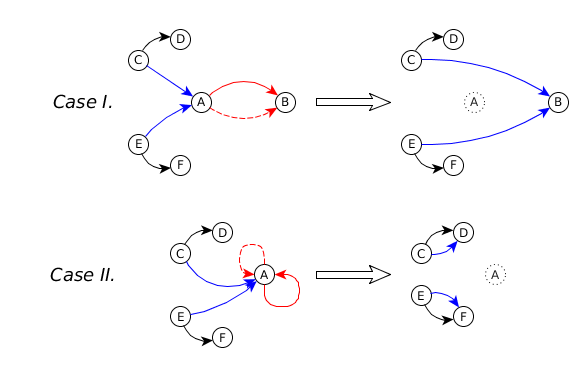
\includegraphics{pruning.png}
\caption{\textbf{Pruning.} Resolution methods for two variations of a (red) prohibited structure.
In both cases, edges originating at node A are eliminated; edges in blue are redirected.
Case II creates two case I-type structures that require further resolution.}
\label{fig:Pruning}
\end{figure}

Both types of changes eliminate the node at which the offending edge pair
originates (labeled "A" in the illustrations), along with the edge pair.
In case I, all edges inbound to the eliminated node are redirected to 
the destination (shown as node "B") of its to-be-eliminated edge pair.
Redirected edges are shown in blue.

Lacking such a natural new destination for the inbound edges in case II, the
pruning process instead moves the problem "upstream"---any edge inbound to
the eliminated node is redirected to the same destination node as that of
its origin node's other out-edge. This, of course, immediately creates
case I structure violations for all such origin nodes; these violations must also be
resolved before the next iteration can begin.
Case II resolutions \textit{always} create additional structure violations;
case I resolutions may or may not. In either case, cascades can result. These
cascades, and the resulting reductions in graph size, are common in both
\textbf{C} and \textbf{R} simulations.

\end{document}
